%----------------------------------------------------------------------------------------
%	Capítulo 6
%----------------------------------------------------------------------------------------

\pagestyle{myportland}
\doublespacing
%\pagenumbering{arabic}
\chapter[\quad\quad\quad\quad ----- Pruebas y resultados]{\\ Pruebas y resultados}
\thispagestyle{myportland}

Este capítulo está enfocado en mostrar simulaciones, pruebas obtenidas de los algoritmos empleados en el sistema. Además desarrolla de manera técnica los resultados con la finalidad de ser comparables con resultados de otros autores de otras máquinas.

%% NUEVA SECCIÓN X.X
\section{Algoritmos de clasificación y conteo de truchas}

Con el fin de realizar la clasificación y conteo se plantea una solución de 4 etapas: detectar, contar, segmentar y medir. Para la primera y segunda etapa, los algoritmos seleccionados para realizar las pruebas son YOLOv3 y YOLOv4\footnote{Se puede probar las demos listadas en la sección \ref{ssec:repositorio de codigo fuente}.} mientras que el conteo se basa en el conteo de truchas detectadas que sobrepasen un umbral mínimo de fiabilidad de (30\%). Para la tercera etapa, se aplica el algoritmo de segmentación llamado GrabCut\footnote{Algoritmo GrabCut: extracción interactiva de primer plano mediante cortes de gráficos iterados \cite{Rother2004}.} que permite quitar el fondo del objeto. Para la cuarta etapa, se usa un objeto referencial con medidas conocidas que permite la medición de la trucha en largo y ancho.

Las bases de datos empleadas en las pruebas para entrenar los algoritmos son la FISH9002 y FISH9003 de elaboración propia que contienen 723 y 2400 imágenes respectivamente. Sin embargo, se muestra únicamente resultados de la base de datos de imágenes FISH9003 ya que es esperable que brinde mejores resultados al brindar una mayor cantidad de imágenes.


% NUEVA SECCIÓN X.X.X
\subsection{Definición de criterios de clasificación}

En la Tabla \ref{tab:matriz de confusion} se muestra la matriz de confusión sobre la cuál se presentan diversas métricas evaluadas en el entrenamiento de los modelos. Los términos técnicos usados son citados de \cite{Everingham2010} y representan métricas para medir el rendimiento, confiabilidad y precisión de los modelos.

\begin{mytable}[H]
	\footnotesize\centering
	\caption{Matriz de confusión.}
	\label{tab:matriz de confusion}
	\begin{tabular}{c|c|c|}
		\cline{2-3}
		& Real Positivo & Real Positivo \\ \hline
		\multicolumn{1}{|c|}{Predecido Positivo} & TP            & FP            \\ \hline
		\multicolumn{1}{|c|}{Predecido Negativo} & FN            & TN            \\ \hline
	\end{tabular}
	\begin{myflushcenteraftertable}	
		Dónde: TP es \textit{True Positive}; FP es \textit{False Positive}; FN es \textit{False Negative}; TN es \textit{True Negative}.
		Fuente: Elaboración propia.
	\end{myflushcenteraftertable}
\end{mytable}

En base a la Tabla \ref{tab:matriz de confusion} se muestran las Ecuaciones \ref{eq:accuracy}, \ref{eq:precision}, \ref{eq:recall}, \ref{eq:f1} y \ref{eq:ap} que son comúnmente usadas para calcular métricas de los modelos. En la siguiente subsección se muestran resultados basados en estas métricas, aunque ninguna es excluyente de otra, aunque la F1 mostrada en la Ecuación \ref{eq:f1} suele ser la principal variable a tomar en cuenta junto con el  map.

\begin{myequation}\label{eq:accuracy}
	\begin{split}
		Accuracy&=\frac{True_{positive}+True_{negative}}{True_{positive}+True_{negative}+False_{positive}+False_{negative}}
	\end{split}
\end{myequation}

\begin{myequation}\label{eq:precision}
	\begin{split}
		Precision&=\frac{True_{positive}}{True_{positive}+False_{positive}}
	\end{split}
\end{myequation}

\begin{myequation}\label{eq:recall}
	\begin{split}
		Recall&=\frac{True_{positive}}{True_{positive}+False_{negative}}
	\end{split}
\end{myequation}

\begin{myequation}\label{eq:f1}
	\begin{split}
		F1&=\frac{2*precision*recall}{precision+recall}
	\end{split}
\end{myequation}

\begin{myequation}\label{eq:ap}
	\begin{split}
		Average Precision&=\int_{0}^{1}p(r)dr
	\end{split}
\end{myequation}

%\vspace{-2.0 em}

% NUEVA SECCIÓN X.X.X
\subsection{Resultados YOLOv3}

En la Figura \ref{fig:resultados yolo 3} se muestra los resultados de entrenamiento del modelo YOLOv3. Dónde: \textit{GIoU} es una métrica que nos permite segmentar mejor la imagen y que conviene se disminuya en el entrenamiento ya que el rectángulo de etiquetado se acerca más al real; \textit{Objectness} es una métrica que nos indica si el modelo detecta correctamente intersecciones, por eso es bueno que disminuya; \textit{Precision} es el ratio entre TP y la suma de TP con FP, que nos indica las veces que el modelo ha detectado bien la cantidad de truchas sobre una imagen; \textit{Recall} es una métrica para medir la capacidad del modelo de detectar TP, mientras es mayor, mientras mayor mejor; \textit{val} se refiere a las métricas en etapa de validación; \textit{mAP@0.5} es la precisión media con mínimo de confiabilidad de 0.5; \textit{F1} es una métrica basada en en el \textit{Recall} y \textit{Precision} que es usado comúnmente junto con la Precision para brindar un balance real de si el modelo funciona correctamente con una precisión adecuada. Como se muestra en la Figura \ref{fig:resultados yolo 3} el modelo tiene una alta precisión pero un score F1 de alrededor de 0.4, esto quiere decir que el modelo logra reconocer truchas pero no de forma esperada.

\begin{myfigure}[H]
	\footnotesize\centering
	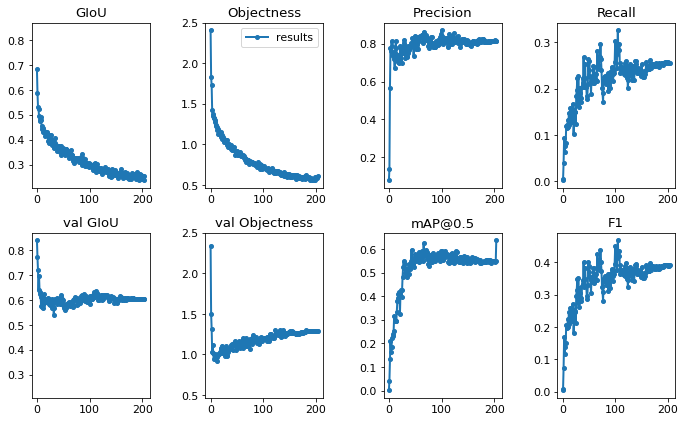
\includegraphics[width=0.85\textwidth]{chapter6/resultados yolo 3.png}
	\caption{Resultados del entrenamiento de YOLOv3.}
	\begin{myflushcenter}
		Fuente: Elaboración propia.
	\end{myflushcenter}
	\label{fig:resultados yolo 3}
\end{myfigure}

% NUEVA SECCIÓN X.X.X
\subsection{Resultados YOLOv4}

En la Figura \ref{fig:resultados yolo 4} se muestra los resultados del entrenamiento del modelo YOLOv4-tiny. En el entrenamiento se registra el \textit{loss} y el \textit{mAP@0.5} \footnote{map: mean average precision, en el caso map@0.5 significa precisión promedio con threshold 0.5.}. El mAP máximo obtenido luego de 2000 iteraciones es de alrededor de 60\% con un score F1 mejor que el obtenido por YOLOv3. Este algoritmo es superior tanto en tiempo de entrenamiento, como en robustez y en tamaño de los pesos de la red (alrededor de 25 MB\footnote{YOLOv3 alrededor de 250 MB.})por lo que se escoge para ser empleado en el sistema.

\begin{myfigure}[H]
	\footnotesize\centering
	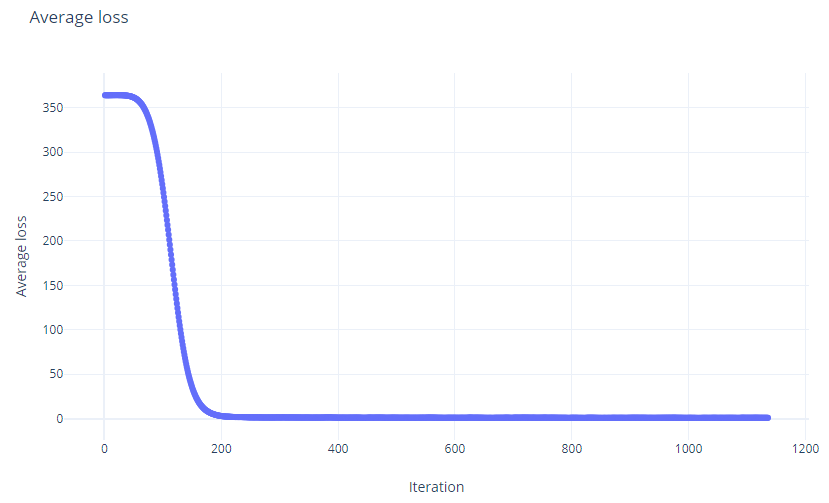
\includegraphics[width=1\textwidth]{chapter6/resultados yolo 4.png}
	\caption{Resultados del entrenamiento de YOLOv4.}
	\begin{myflushcenter}
		Fuente: Elaboración propia.
	\end{myflushcenter}
	\label{fig:resultados yolo 4}
\end{myfigure}


% NUEVA SECCIÓN X.X.X
\subsection{Resultados del algoritmo de detección}

Luego de detectado el objeto se procede a segmentarlo mediante técnicas de enmascarado de objetos. Finalmente cada objeto detectado en la imagen es contabilizado dentro del programa. En la Figura \ref{fig:pruebas algoritmo} se muestra en el lado izquierdo la imagen que se ingresa al algoritmo y a la derecha el pez segmentado contabilizado.

\begin{myfigure}[H]
	\footnotesize\centering
	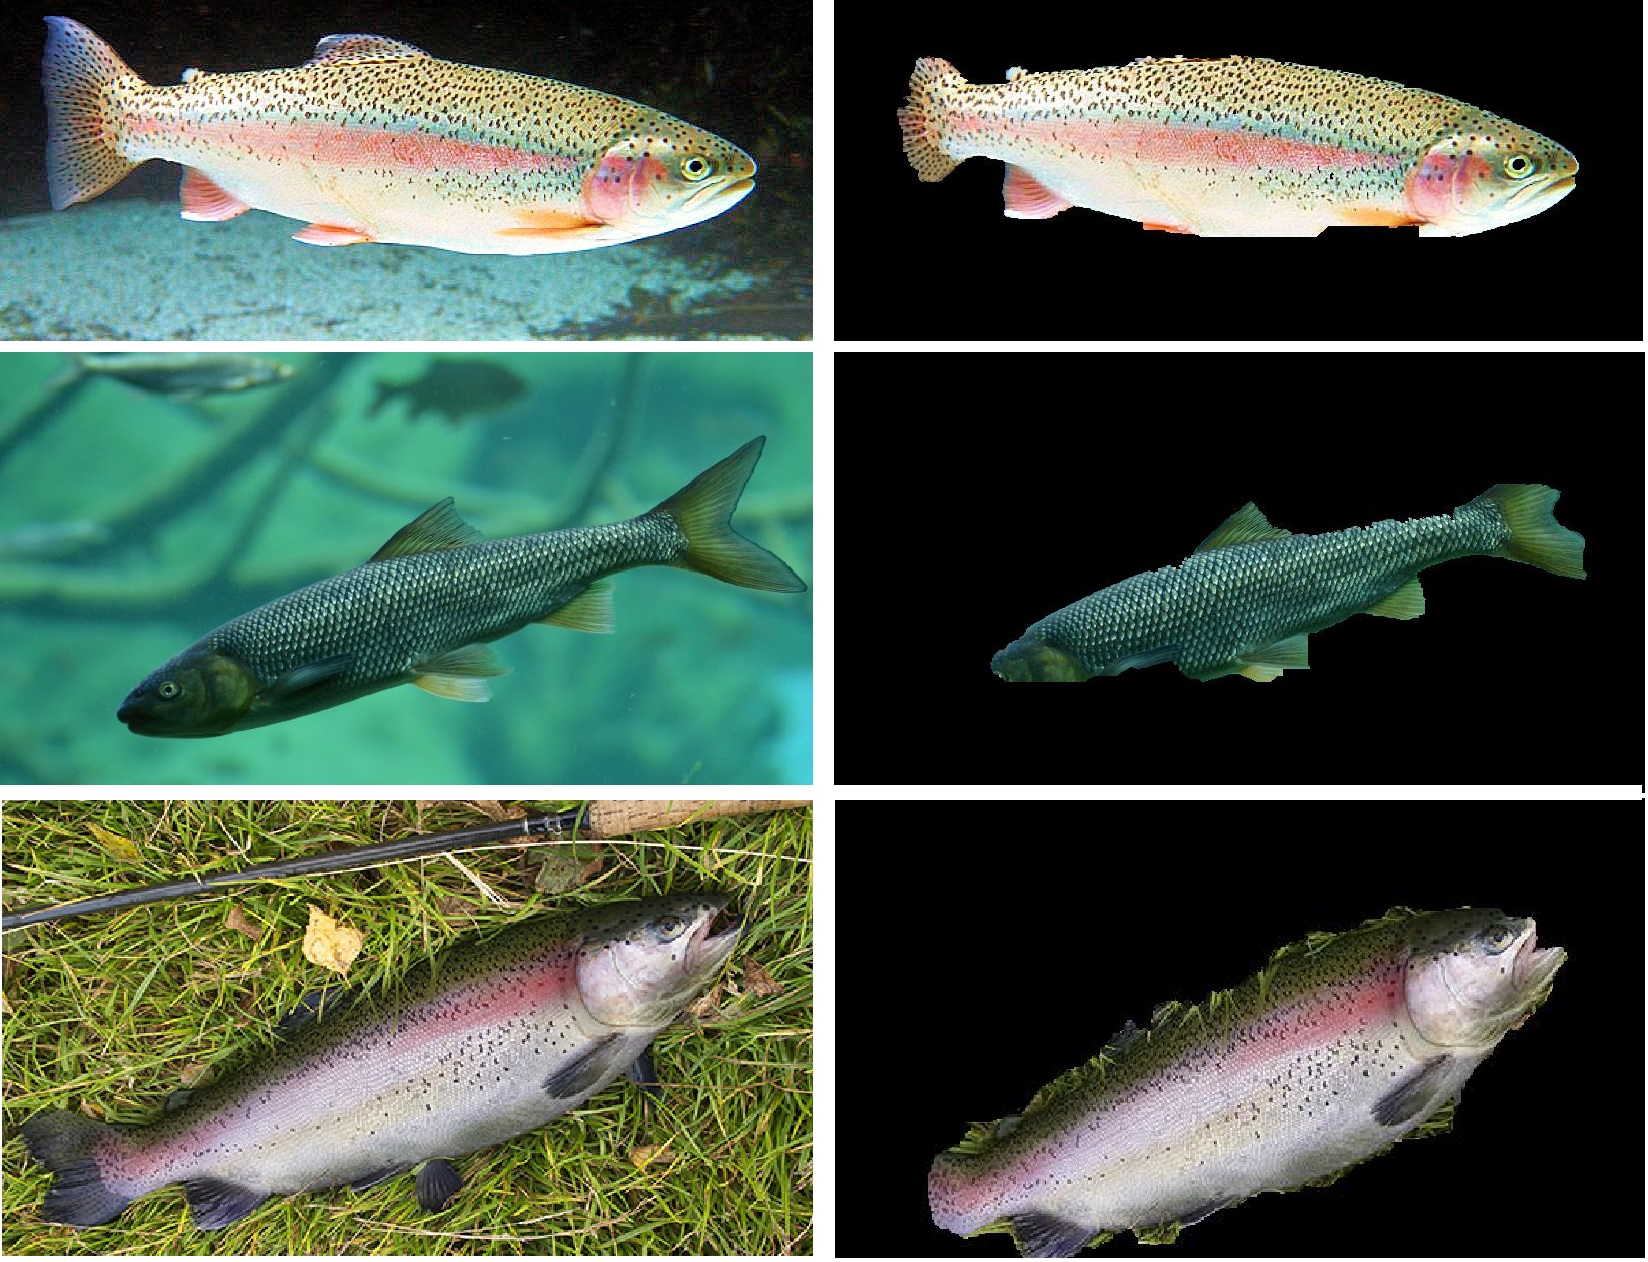
\includegraphics[width=1\textwidth]{chapter6/pruebas algoritmo.png}
	\caption{Inferencia de detección y conteo de truchas.}
	\begin{myflushcenter}
		Fuente: Elaboración propia.
	\end{myflushcenter}
	\label{fig:pruebas algoritmo}
\end{myfigure}

En el caso de la clasificación el sistema debe ser calibrado acorde al entorno, por lo que su etapa de desarrollo luego de la detección se da en la etapa de prototipado y producción. Sin embargo, el conteo es realizado sin ningún problema.


% NUEVA SECCIÓN X.X.X
\subsection{Tiempos de ejecución y detección}

De los algoritmos propuestos, YOLOv3 se entrenó en Google Colab\footnote{Servicio gratuito de google para deep learning. Brinda GPUs de forma gratuita.} con una GPU Tesla T4 como se muestra en la Figura \ref{fig:colab}. En cuánto a la versión 3 del algoritmo, en el entrenamiento el algoritmo procesó alrededor de 12 horas los pesos de la red. Por el contrario, con la versión 4 del algoritmo con modificación de escalamiento llamado tiny, el proceso demoró alrededor de una hora brindando resultados excelentes que se muestran en la subsección anterior.\footnote{Los códigos usados para entrenar los modelos se encuentran listados en la sección de \ref{ssec:repositorio de codigo fuente}.} El tiempo de inferencia es el tiempo que requiere procesar cada capa dentro de la arquitectura de red neuronal de cada algoritmo, mientras más capas posee la arquitectura, suele tomar mayor tiempo de inferencia. Sin embargo, hay mecanismos que permiten optimizar el tiempo de inferencia, estos mecanismos son aplicados en YOLOv3 y YOLOv4 respecto a YOLOv1 que hacen que el tiempo de inferencia para imágenes de 416x416 pixeles sea mucho menor. En el caso de YOLOv3 el $t_{inf}=0.06 s$, mientras que para YOLOv3 el $t_{inf}=0.0083 s$. Con el último modelo se puede conseguir hasta 120 fps de procesamiento en un video con 3 canales de color, si esto se reduce únicamente al canal B/N\footnote{B/N: Blanco y negro.} decrementa aún más.\footnote{Investigaciones recientes no publicadas muestran resultados de hasta 320 fps.}.

\begin{myfigure}[H]
	\footnotesize\centering
	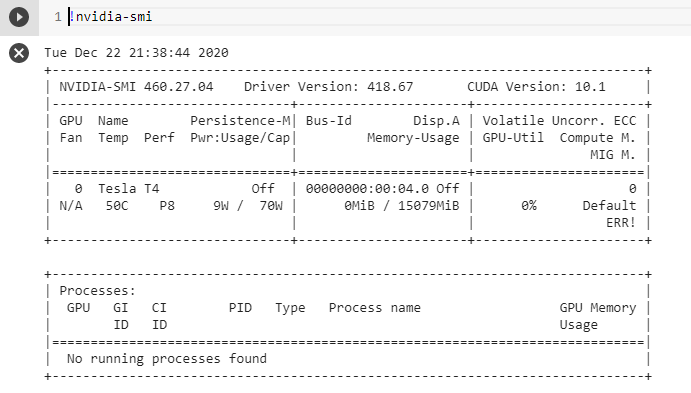
\includegraphics[width=0.75\textwidth]{chapter6/colab.png}
	\caption{Tarjeta gráfica (GPU) usada en el entrenamiento de YOLOv3 y YOLOv4.}
	\begin{myflushcenter}
		Fuente: Elaboración propia.
	\end{myflushcenter}
	\label{fig:colab}
\end{myfigure}

%% NUEVA SECCIÓN X.X
\section{Algoritmo de medición}


El algoritmo de medición se calibra digitalmente mediante un objeto dentro de la imagen.\footnote{Autor del algoritmo: PyImageSearch} En la Figura \ref{fig:medicion} se muestra la dimensión del sol peruano y la dimensión de la trucha en base a esa dimensión de la moneda. El algoritmo aplica filtros para diferenciar el fondo de los objetos, luego detecta el objeto más a la izquierda y le brinda las medidas que se brinda mediante línea de código\footnote{Más información en el repositorio listado en la sección \ref{ssec:repositorio de codigo fuente}.}, luego encierra los objetos con las dimensiones calculadas en rectángulos. Finalmente, se muestran las dimensiones sobre la imagen como se muestra en la Figura \ref{fig:medicion}.\footnote{La tabla de clasificación de truchas en base a su tamaño se citan en \cite{DiazVergara2020}.}

\begin{myfigure}[H]
	\footnotesize\centering
	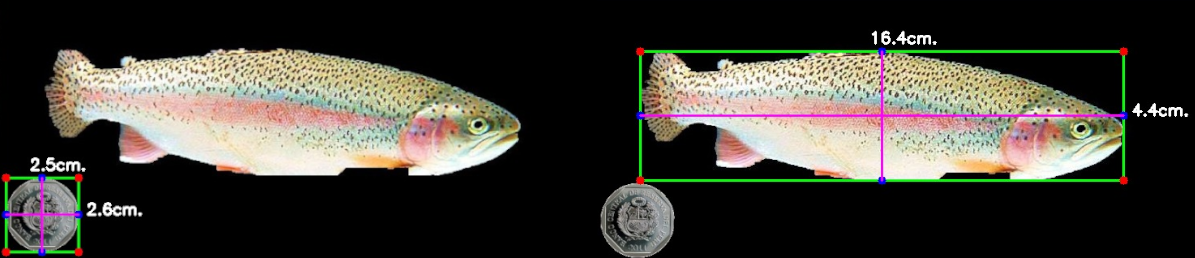
\includegraphics[width=1\textwidth]{chapter6/medicion truchas.png}
	\caption{Medición digital de una trucha referenciada dimensionalmente con una moneda de 1 sol peruano.}
	\begin{myflushcenter}
		Fuente: Elaboración propia.
	\end{myflushcenter}
	\label{fig:medicion}
\end{myfigure}

%% NUEVA SECCIÓN X.X
\section{Simulación estructural}

Las simulaciones estructurales se realizan dentro de softwares que permiten simular fuerzas, momentos y esfuerzos a los que se estima estará sometido los componentes mecánicos del sistema.

%% NUEVA SECCIÓN X.X.X
\subsection{Armadura}

La armadura de soporte hecha de perfiles cuadrados de acero inoxidable con norma ISO 316 tiene un factor de seguridad (F.S.) de sometido a las fuerzas presentes del sistema. En La Figura \ref{fig:simulacion armadura} se muestra un mapa de calor que muestra el factor de seguridad según la zona de la armadura. Como se muestra en la Figura  \ref{fig:simulacion armadura} el factor mínimo de seguridad es 15, por lo que se garantiza la integridad de la armadura sometida a las fuerzas y cargas esperadas.

\begin{myfigure}[H]
	\footnotesize\centering
	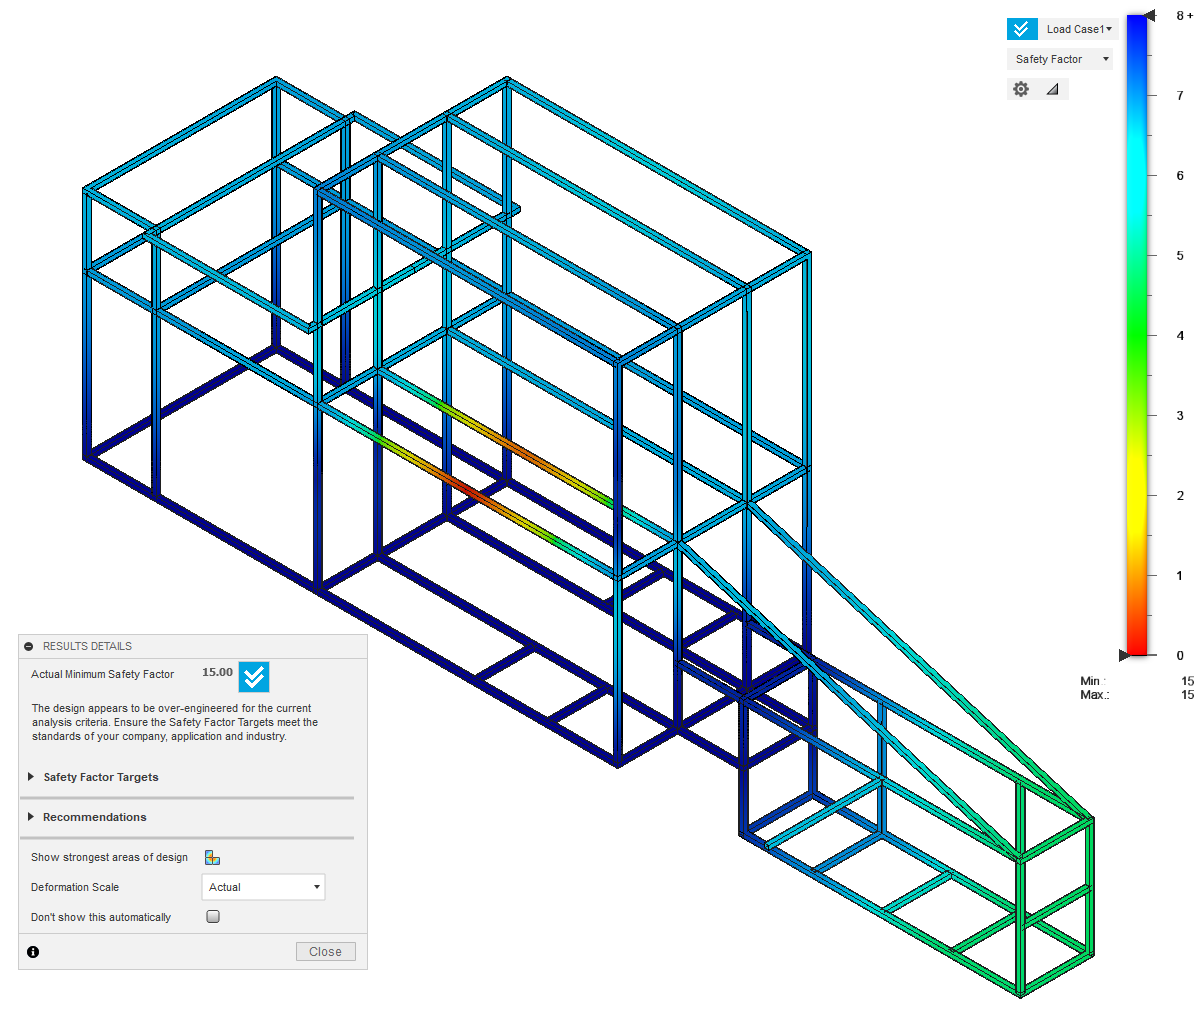
\includegraphics[width=1\textwidth]{chapter6/simulacion armadura.png}
	\caption{Cálculo de factor de seguridad de armadura en operación.}
	\begin{myflushcenter}
		Fuente: Elaboración propia.
	\end{myflushcenter}
	\label{fig:simulacion armadura}
\end{myfigure}


%% NUEVA SECCIÓN X.X.X
\subsection{Plataforma flotante}

Un componente clave a pesar de no estar dentro del diseño directo del sistema es la plataforma sobre la cual el sistema se apoya para ser estable en medio de un lago o laguna. La plataforma flotante fue diseñada y simulada bajo cargas de hasta 300 kilos repartidas en una área que ocupa el sistema que se propone. En la Figura \ref{fig:simulacion plataforma} se muestra que el factor de seguridad del sistema es de 15 lo cual nos indica que la plataforma soportará la carga sin problemas y no es riesgo para su flotabilidad.

\begin{myfigure}[H]
	\footnotesize\centering
	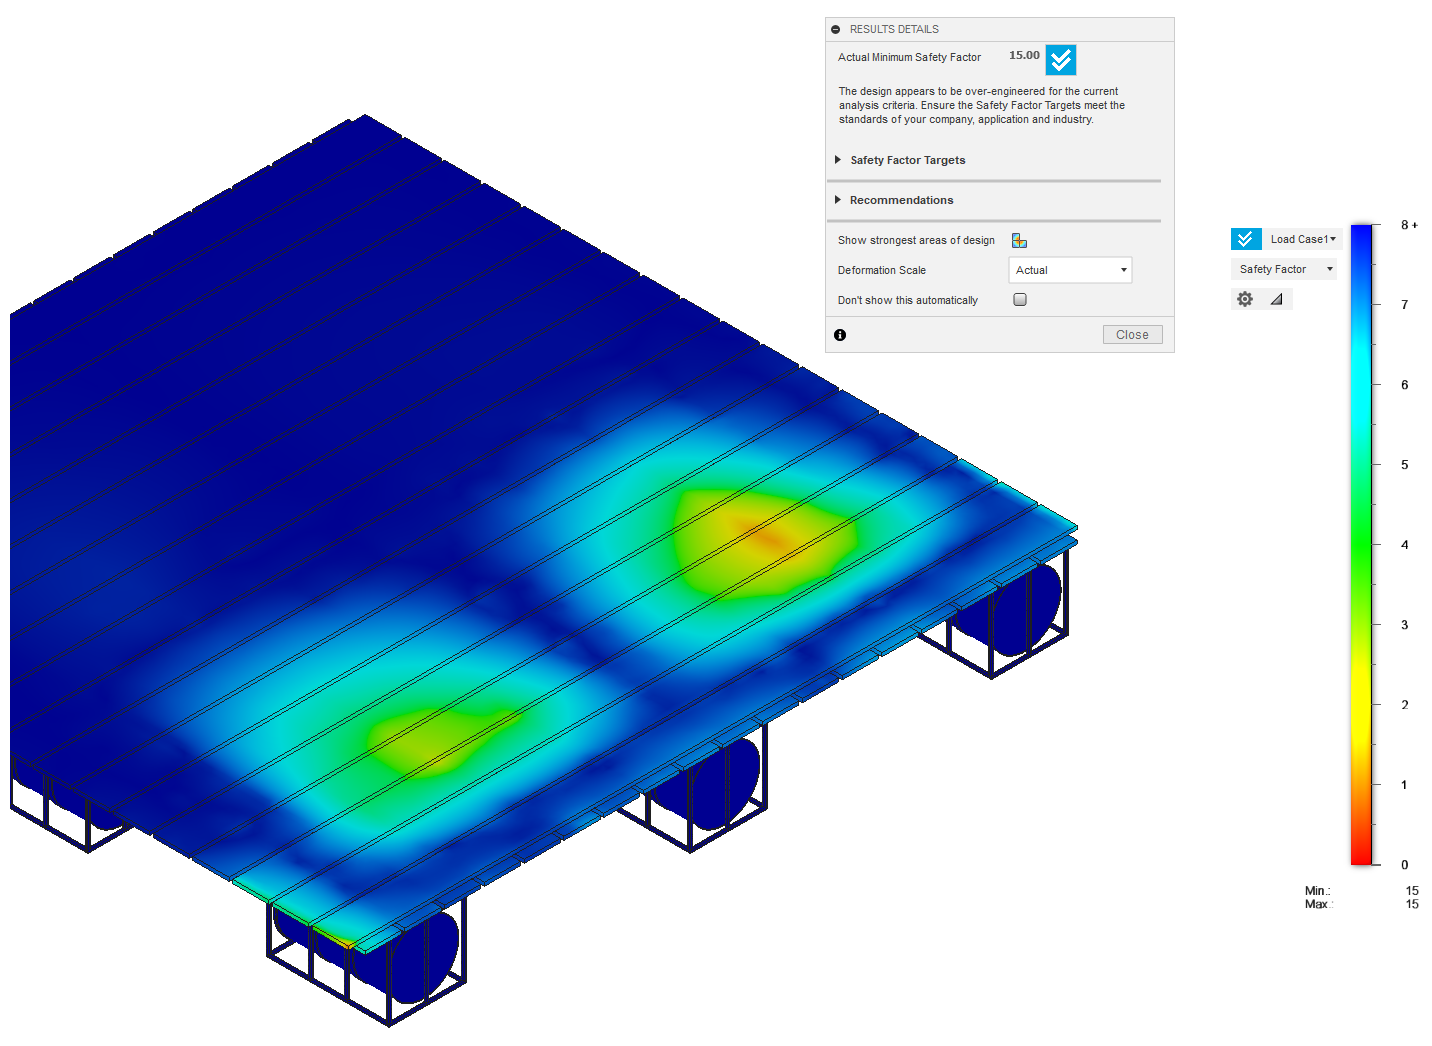
\includegraphics[width=1\textwidth]{chapter6/simulacion plataforma.png}
	\caption{Cálculo de factor de seguridad en la plataforma flotante de 5x5 m.}
	\begin{myflushcenter}
		Fuente: Elaboración propia.
	\end{myflushcenter}
	\label{fig:simulacion plataforma}
\end{myfigure}


%% NUEVA SECCIÓN X.X.X
%\subsection{Distribuidora de truchas}


%La distribuidora de truchas se elabora principalmente con procesos de plegado de metales, en este caso acero inoxidable AISI 316 y una placa de PMMA. La distribuidora no está sujeta a tensiones, compresiones o esfuerzos considerables, la única carga que posee es la de la trucha en tránsito. Por lo que se estudia la carga de la trucha dentro de sus compartimentos. En la Figura \ref{fig:simulacion distribuidora} se muestra un mapa de calor que muestra el factor de seguridad según la zona de la armadura.

%\begin{myfigure}[H]
%	\footnotesize\centering
%	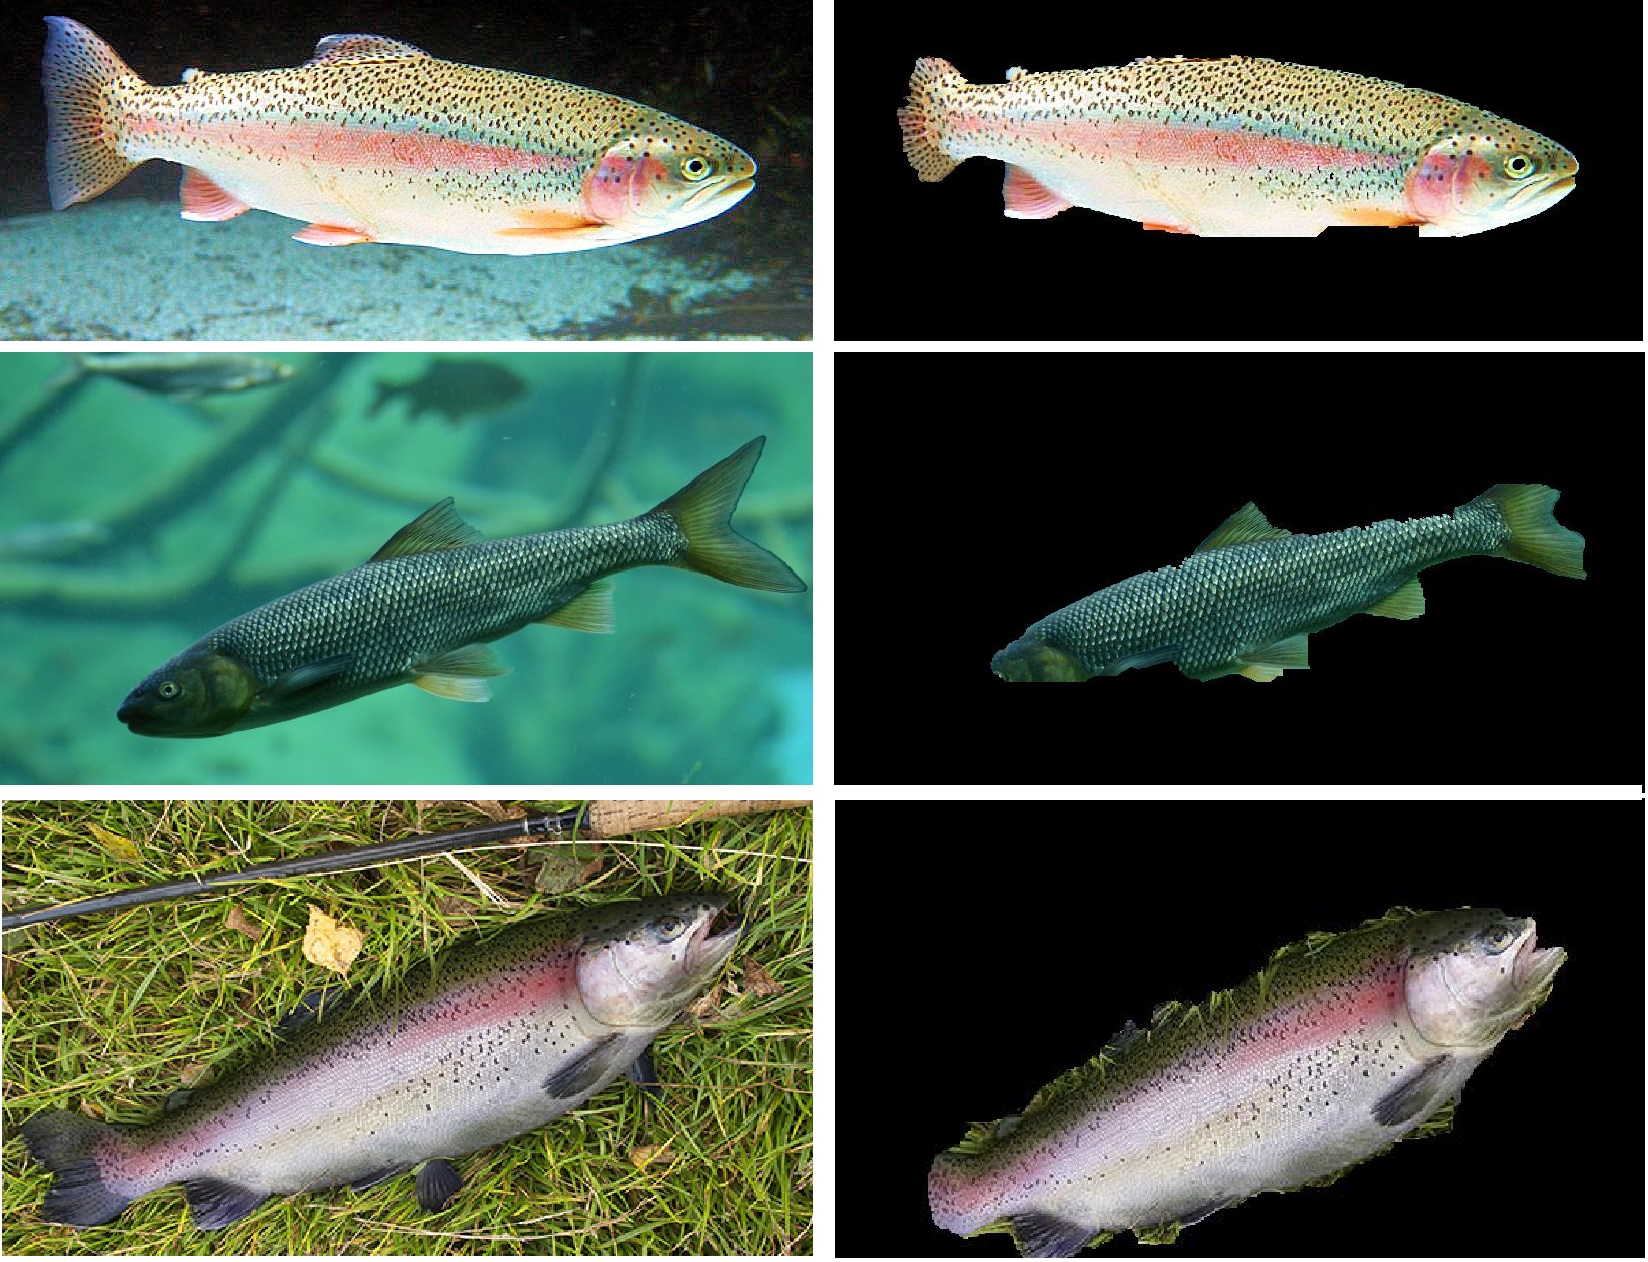
\includegraphics[width=1\textwidth]{chapter6/simulacion distribuidora.png}
%	\caption{Cálculo de factor de seguridad en la distribuidora de truchas.}
%	\begin{myflushcenter}
%		Fuente: Elaboración propia.
%	\end{myflushcenter}
%	\label{fig:simulacion distribuidora}
%\end{myfigure}